\documentclass[conference]{IEEEtran}
\IEEEoverridecommandlockouts
\usepackage{cite}
\usepackage{balance}
\usepackage{amsmath,amssymb,amsfonts}
\usepackage{graphicx}
\usepackage{textcomp}
\usepackage{xcolor}
\usepackage{booktabs}
\usepackage{tikz}
\usetikzlibrary{positioning,arrows.meta,fit}
\usepackage[hidelinks]{hyperref}

\begin{document}

\title{Fail-Closed Flood Evacuation Decision Support:\\
Gauge-Held-Out Forecasting and a Constraint\\
Shield for Learned Route Proposals}

\author{\IEEEauthorblockN{Anonymous Author(s)}
\IEEEauthorblockA{\textit{Affiliation withheld for double-blind review}}}

\maketitle

\begin{abstract}
Flood evacuation tools usually treat forecasting, decision making and routing as separate problems, and they are often evaluated in ways that hide their failure modes. We present a flood decision-support system in which every stage either produces an auditable result or hands control to a human operator. The forecasting stage predicts whether streamflow will exceed a gauge's 95th-percentile flow within three days. Trained on 242 CAMELS-IND gauges and tested on 49 gauges held out in both space and time (2015--2020), an XGBoost model reached a balanced accuracy of 0.898 and ROC-AUC of 0.965, against 0.765 and 0.765 for a persistence baseline; its precision of 0.328 remains the main weakness. The decision stage maps risk to monitor, human-review or automated-response actions and falls back to review whenever data, model or database health checks fail. The routing stage places a constraint shield, formulated as a quadratic unconstrained binary optimization (QUBO) feasibility filter followed by a deterministic validator, after an adaptive route proposer. Across 90 seeded scenarios with injected road closures and shelter overload, the shield raised the proposer's safe-route rate from 68.3\% to 93.3\% under four closures and eliminated capacity violations. It did not outperform flood-aware A*, and we report that result directly. We also show that a gate based on mean source reliability fails to trigger on most single-source failures.
\end{abstract}

\begin{IEEEkeywords}
flood forecasting, evacuation routing, safe reinforcement learning, shielding, QUBO, human-in-the-loop, digital twin
\end{IEEEkeywords}

\section{Introduction}
Floods are among the most damaging natural hazards in India, and during a monsoon event the questions an emergency officer must answer change by the hour: will this river cross its warning level in the next few days, should evacuation start now or wait for review, and which roads and shelters are still usable? Machine-learning forecasters have become good at the first question, even in basins without long records \cite{Nearing2024}, and graph search answers the last one quickly. What is less settled is how these pieces should be joined so that a wrong or stale input cannot silently turn into a dispatch order.

Learned route policies make this concern sharper. Reinforcement learning (RL) has been applied to evacuation planning for storm surge \cite{LiuC2025} and wildfire \cite{Raei2026}, and it can anticipate congestion that a shortest-path search ignores. A policy trained with reward penalties, however, still has no guarantee that it will avoid a closed bridge or a full shelter at run time. The safe-RL literature addresses this with \emph{shields} that block unsafe actions before they reach the environment \cite{Alshiekh2018,Garcia2015}. To our knowledge, this idea has not been evaluated in a flood-evacuation setting alongside the forecasting and gating stages that feed it.

This paper describes and evaluates such a pipeline, built as an open full-stack prototype. Our contributions are:
\begin{enumerate}
\item A fail-closed decision chain in which a hazard-monotone risk score drives a three-way policy (monitor, human review, automated response), and any failed data, model or database health check downgrades automation to review.
\item A proposer-agnostic constraint shield for evacuation routes, with closures, shelter capacity, vehicles and accessibility encoded as QUBO penalties, plus a deterministic validator that re-checks the final plan.
\item A leakage-controlled evaluation of three-day flood-exceedance forecasting on CAMELS-IND gauges that are unseen in both space and time, reported against a persistence baseline.
\item A seeded stress test of the shield and of reliability gating, including results that do not favour our design.
\end{enumerate}
We make no claim of quantum speed-up. The QUBO form is used because it expresses hard constraints as penalties that any binary solver can consume. In this prototype it is solved classically.

\section{Related Work}
\textit{Flood forecasting.} Tree ensembles, support vector machines and neural networks are widely used for flood susceptibility and prediction \cite{Mosavi2018}. Nearing \textit{et al.} showed that a model trained on thousands of gauges forecasts extreme floods in ungauged basins with skill comparable to an operational physical system \cite{Nearing2024}. Graph-based models that encode river topology have since reported longer warning lead times \cite{Kirschstein2024}. For India, CAMELS-IND provides daily forcing, streamflow and catchment attributes for 228 peninsular catchments \cite{Mangukiya2025}, and INDOFLOODS catalogues historical flood events \cite{Kuntla2025}. Many published models are validated with random row splits. When neighbouring days from the same gauge fall on both sides of the split, accuracy is inflated, so we hold out whole gauges and later years.

\textit{Evacuation routing and learning.} Classical formulations use shortest paths, network flows or vehicle routing, with Dijkstra \cite{Dijkstra1959}, A* \cite{Hart1968} and $k$-shortest paths \cite{Yen1971} as building blocks. Deep Q-networks and policy-gradient methods such as PPO \cite{Schulman2017} have been used to learn evacuation policies \cite{LiuC2025,Raei2026}. Shielding \cite{Alshiekh2018} and related constrained-RL methods \cite{Garcia2015} correct a policy's action at run time instead of relying on the reward to discourage violations.

\textit{Binary optimization.} Assignment and routing constraints can be written as Ising or QUBO models \cite{Lucas2014} and solved by simulated annealing \cite{Kirkpatrick1983}, quantum annealing \cite{Cadelina2024} or the Quantum Approximate Optimization Algorithm (QAOA) \cite{Farhi2014}. We use the QUBO form for its constraint encoding, not for any expected hardware advantage.

\textit{Explanation and digital twins.} SHAP attributes a prediction to its inputs \cite{Lundberg2017}, and TreeSHAP computes exact values for tree ensembles \cite{Lundberg2020}. Feature attributions cannot by themselves tell an officer that a route was rejected because a bridge is closed, so we pair them with explicit constraint traces. Practitioners co-designing a flood digital twin ranked data provenance and transparent ``what-if'' runs above visual realism \cite{Underhill2026}. This finding shaped our rule that simulated data is always labelled as simulated.

\section{System Overview}
Fig.~\ref{fig:arch} shows the pipeline. A FastAPI backend runs one function, \texttt{run\_pipeline(mode, observations)}, in both live mode, which uses Open-Meteo weather and river discharge data, and simulation mode, which uses a digital twin of the Delhi Yamuna corridor and five reservoirs. Live and simulated snapshots are stored separately in MongoDB, so a synthetic tick can never appear on the live dashboard. A React interface reads every displayed value from this state.

\begin{figure}[t]
\centering
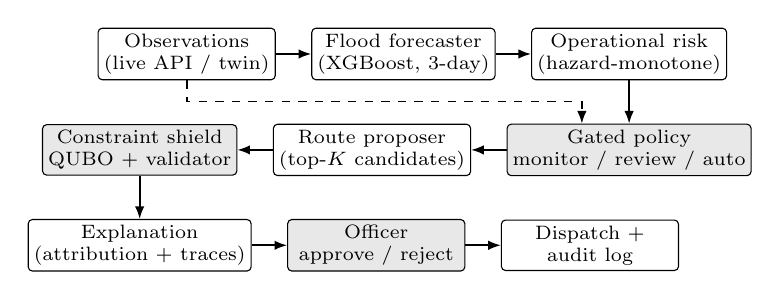
\begin{tikzpicture}[
  font=\scriptsize,
  box/.style={draw, rounded corners=1.5pt, align=center, minimum width=2.25cm, minimum height=0.62cm, inner sep=2pt},
  gate/.style={box, fill=gray!18},
  arr/.style={-{Latex[length=1.6mm]}, semithick}]
\node[box] (obs) {Observations\\(live API / twin)};
\node[box, right=0.45cm of obs] (fc) {Flood forecaster\\(XGBoost, 3-day)};
\node[box, right=0.45cm of fc] (risk) {Operational risk\\(hazard-monotone)};
\node[gate, below=0.55cm of risk] (pol) {Gated policy\\monitor / review / auto};
\node[box, left=0.45cm of pol] (prop) {Route proposer\\(top-$K$ candidates)};
\node[gate, left=0.45cm of prop] (shield) {Constraint shield\\QUBO + validator};
\node[box, below=0.55cm of shield] (xai) {Explanation\\(attribution + traces)};
\node[gate, right=0.45cm of xai] (hum) {Officer\\approve / reject};
\node[box, right=0.45cm of hum] (out) {Dispatch +\\audit log};
\draw[arr] (obs) -- (fc);
\draw[arr] (fc) -- (risk);
\draw[arr] (risk) -- (pol);
\draw[arr] (pol) -- (prop);
\draw[arr] (prop) -- (shield);
\draw[arr] (shield) -- (xai);
\draw[arr] (xai) -- (hum);
\draw[arr] (hum) -- (out);
\draw[arr, dashed] (obs.south) -- ++(0,-0.27) -| ([xshift=-6mm]pol.north);
\end{tikzpicture}
\caption{Fail-closed pipeline. Shaded blocks can stop or downgrade automation. The dashed link carries source reliability and health checks to the policy. Every block writes to the audit log.}
\label{fig:arch}
\end{figure}

\subsection{Forecasting Stage}
For gauge $g$ on day $t$, the target is
\begin{equation}
y_{g,t}=\mathbf{1}\Big[\max_{h\in\{1,2,3\}} Q_{g,t+h}\ \ge\ q^{95}_{g}\Big],
\label{eq:target}
\end{equation}
where $Q$ is observed streamflow and $q^{95}_{g}$ is the gauge's 95th-percentile flow over the training years 1980--2008 only. The model uses 50 inputs: lagged and accumulated rainfall (up to 90 days), temperature, humidity, evapotranspiration, four soil-moisture layers, lagged and rolling streamflow, seasonality, and static catchment attributes such as area, slope, aridity and land cover. Hydrological signatures in CAMELS-IND are excluded because they are computed over the full record, including the test years. Future rainfall is also excluded.

\subsection{Risk and Gated Decision Policy}
The live risk engine combines a model prior $p_{\mathrm{ML}}$ with two hazard terms:
\begin{equation}
p=\operatorname{clip}\big(0.16+0.50\,\sigma_R+0.20\,h_S+0.14\,p_{\mathrm{ML}},\,0,\,1\big),
\label{eq:risk}
\end{equation}
with $\sigma_R=1/(1+e^{-(R-38)/12})$ for 24-h rainfall $R$ in mm, and $h_S$ the mean of $\operatorname{clip}((s-70)/30,0,1)$ over river and dam stages $s$, each expressed as a percentage of its danger level. The coefficients are fixed design choices rather than learned values, and a unit test checks that $p$ never falls as rainfall rises. The policy returns \textsc{monitor} for $p<0.50$ and \textsc{human review} for $0.50\le p<0.60$. It returns \textsc{automated response} for $p\ge0.60$ only when the data-quality, model-health and database-health checks all pass; otherwise the action is downgraded to review and the reason is logged. Thresholds live in a single configuration module served over the API, so the interface and backend cannot disagree.

\subsection{Route Proposer and Constraint Shield}
The routing study uses a 15-node network with three population zones, nine junctions, three shelters and 22 roads. Each road carries a travel time, flood depth index and congestion level. Candidate routes come from Yen's $k$-shortest paths on two graphs: the open-road graph and a graph that still contains closed roads. Including closed roads imitates a learned policy that has not yet seen a closure. The proposer ranks candidates by $w_T T + w_H H$, where $T$ is travel time and $H$ is hazard exposure, adjusted by group priority. It updates $w_T$ and $w_H$ online from a reward that penalises hazard and infeasibility. This is a lightweight adaptive policy, not a trained deep PPO agent. The shield treats it as a black box, so a trained agent can replace it without changing the interface.

Let $x_k\in\{0,1\}$ select candidate $k$ for a group. The shield builds
\begin{equation}
E(\mathbf{x})=\sum_k c_k x_k + P_1\Big(1-\sum_k x_k\Big)^2 + P_2\sum_k v_k x_k ,
\label{eq:qubo}
\end{equation}
where $c_k=T_k+5H_k$ is the route cost, the second term enforces a one-hot choice, and $v_k$ counts violations of four hard constraints: closed roads, remaining shelter seats, available vehicles and accessibility for vulnerable groups. The penalties are set so that $P_2>\max_k c_k$, which guarantees that a feasible route always has lower energy than an infeasible one. Candidates with $v_k>0$ are removed before solving. The remaining one-hot problem is solved by simulated annealing, and a QAOA-inspired classical sampler is run alongside for comparison. A deterministic validator then re-checks the chosen route against the current graph version, shelter seats, vehicles, accessibility and data freshness. If the graph changed during solving, the result is discarded.

\subsection{Reliability Gating and Explanations}
Each data source (weather, flood sensor, radar, road database and citizen reports) has a reliability value set by its status. For example, live sources start at 0.88--0.94, a stale road feed drops to 0.40, and a drifting sensor drops to 0.48. Automatic dispatch is blocked when the mean reliability falls below 0.60 or when a cross-source conflict score reaches 0.55. In the present prototype, the conflict score comes from a scripted scenario (Section~\ref{sec:gating}) rather than being estimated from data. Every recommendation carries two explanations: attribution bars over travel time, hazard, congestion, shelter seats, reliability and priority, and a trace listing each rejected candidate with the constraint it broke. For the flood forecaster, TreeSHAP is computed on the same booster that produced the displayed probability.

\section{Experimental Setup}
\textit{Forecasting.} The data cover 242 CAMELS-IND gauges. Training uses 1,641,197 gauge-days from 1980--2008 and validation uses 349,645 gauge-days from 2009--2014, all from gauges seen in training. The primary test set holds out 49 gauges, 20\% of the total, with a group split (seed 42); 48 of them have observations in 2015--2020, giving 52,994 gauge-days that were never used for training or tuning. Seven candidate models (logistic regression, random forest, histogram gradient boosting and four XGBoost \cite{Chen2016} configurations) were compared on validation balanced accuracy. The decision threshold, 0.45, was also chosen on validation. The test set was used once.

\textit{Metrics.} Floods occur on few days, so accuracy is misleading. We report the balanced accuracy
\begin{equation}
\mathrm{BA}=\tfrac12\Big(\frac{TP}{TP+FN}+\frac{TN}{TN+FP}\Big),
\label{eq:ba}
\end{equation}
together with precision, recall, F1, ROC-AUC and the area under the precision--recall curve (PR-AUC), which is sensitive to false alarms on rare events. For routing, let $s^{(1)}_i$ and $s^{(2)}_i$ be 1 when the initial and the re-planned route of scenario $i$ pass every hard check and 0 otherwise. The safe-route rate over $N$ scenarios is
\begin{equation}
S=\frac{100}{N}\sum_{i=1}^{N}\tfrac12\big(s^{(1)}_i+s^{(2)}_i\big).
\label{eq:safe}
\end{equation}
We also report the travel time of the final route, the number of plans that exceed shelter capacity and the wall-clock re-planning latency.

\textit{Routing.} Each scenario draws flood depths, congestion, shelter occupancy and group sizes from a fixed seed ($42+17i$, $i=0,\dots,29$). A route is planned, road R5 is then closed, and Shelter A receives 50\% of its capacity as new arrivals. The route is then re-planned. A plan is \emph{safe} if both the initial and re-planned routes avoid closed roads and satisfy capacity, vehicle and accessibility checks. We compare six methods: static shortest path by distance, flood-aware A*, a risk-aware greedy search, the proposer alone, the proposer with the shield solved by simulated annealing, and the proposer with the shield solved by the QAOA-inspired sampler. The stress test repeats the 30 scenarios with 0, 2 and 4 additional random closures (90 scenarios per method). It also varies the flood-severity setting over 0.20, 0.35, 0.50 and 0.65. Latencies were measured on a consumer laptop and include only the Python planning code.

\textit{Reproducibility.} Every routing and gating number in this paper comes from one script that runs the prototype's own planning engine with fixed seeds and writes its results to a single file, and a build step fails if any number in the text differs from that file or from the stored forecasting evaluation. The forecasting split, the selected model and its threshold are stored with the model, so the test-set figures can be recomputed without retraining. Latencies are the only values that change from run to run, and we report them as indicative.

\section{Results}

\subsection{Forecasting on Unseen Gauges}
Table~\ref{tab:fc} summarises test performance. Floods occur on 5.5\% of test days, so a model that always predicts ``no flood'' would be 94.5\% accurate. For this reason we report balanced accuracy and precision--recall measures. The model found 90.2\% of flood windows at gauges it had never seen, compared with 53.8\% for persistence. Its ranking quality was also higher, with a PR-AUC of 0.737 against 0.449. The cost is false alarms: precision is 0.328, and its F1 score is lower than persistence. When we keep only windows in which the river was below threshold on day $t$, a stricter onset test, recall falls to 0.813 and PR-AUC to 0.369. On validation, the seven candidates were close (balanced accuracy 0.899--0.911), so the choice of model mattered less than the features and the split.

\begin{table}[t]
\caption{Three-day exceedance forecasting on 48 unseen gauges, 2015--2020}
\label{tab:fc}
\centering
\footnotesize
\setlength{\tabcolsep}{2.3pt}
\begin{tabular}{lcccccc}
\toprule
Method & BA & Recall & Prec. & F1 & ROC-AUC & PR-AUC\\
\midrule
Persistence & 0.765 & 0.538 & \textbf{0.789} & \textbf{0.640} & 0.765 & 0.449\\
XGBoost (all days) & \textbf{0.898} & \textbf{0.902} & 0.328 & 0.481 & \textbf{0.965} & \textbf{0.737}\\
XGBoost (onsets) & 0.857 & 0.813 & 0.177 & 0.290 & 0.940 & 0.369\\
\bottomrule
\multicolumn{7}{l}{\scriptsize BA = balanced accuracy; threshold 0.45 (set on validation); $n$ = 52,994.}
\end{tabular}
\end{table}

Table~\ref{tab:val} lists the validation results that drove model selection. Logistic regression, fitted on a 500,000-row subsample, was only 0.012 below the selected model in balanced accuracy. The tree ensembles differed by at most 0.006, and depth had almost no effect. The selected configuration, a depth-6 XGBoost model refitted on all training rows, had the highest balanced accuracy and PR-AUC on validation. Every candidate had a validation precision between 0.391 and 0.420, so the low precision comes from the task and the threshold rule and appears in every model family.

\begin{table}[t]
\caption{Validation results of the seven candidates (2009--2014, $n$ = 349,645)}
\label{tab:val}
\centering
\footnotesize
\setlength{\tabcolsep}{3pt}
\begin{tabular}{llcccc}
\toprule
Model & Rows & BA & Recall & Prec. & PR-AUC\\
\midrule
Logistic regression & sub & 0.899 & 0.916 & 0.391 & 0.751\\
Random forest & sub & 0.905 & 0.924 & 0.403 & 0.781\\
Hist. gradient boosting & full & 0.909 & 0.930 & 0.408 & 0.791\\
XGBoost, depth 4 & full & 0.909 & 0.934 & 0.401 & 0.790\\
XGBoost, depth 6 (earlier fit) & full & 0.909 & 0.925 & 0.420 & 0.792\\
XGBoost, depth 8 & full & 0.909 & 0.927 & 0.416 & 0.793\\
XGBoost, depth 6 (selected) & full & \textbf{0.911} & \textbf{0.936} & 0.404 & \textbf{0.796}\\
\bottomrule
\multicolumn{6}{l}{\scriptsize sub = 500,000-row training subsample; full = all 1,641,197 training rows.}\\
\end{tabular}
\end{table}

\subsection{Where the Forecaster Works and Where It Fails}
To check that the reported scores belong to the saved model, we re-scored the stored test set with it and obtained the same balanced accuracy (0.898), ROC-AUC (0.965) and PR-AUC (0.737). Fig.~\ref{fig:curves} shows the full precision--recall and ROC curves. Persistence lies almost exactly on the model's precision--recall curve: at persistence's recall of 0.538, the model's best precision is 0.786, against 0.789 for persistence. At that operating point the two are equivalent. The model's advantage is that it can also operate at much higher recall, and the curve shows that this is bought with many more false alarms.

\begin{figure}[t]
\centering
\includegraphics[width=\columnwidth]{fig_curves.pdf}
\caption{Precision--recall (left) and ROC (right) curves on the 48 unseen test gauges. The square is persistence; the dotted line on the left is the flood rate.}
\label{fig:curves}
\end{figure}

Pooled scores can hide gauges where the model fails. Of the 48 test gauges, 46 had at least one flood window in 2015--2020. Their balanced accuracies (Fig.~\ref{fig:gauges}) had a median of 0.900 and an interquartile range of 0.860--0.926. The worst gauge reached 0.769, and no gauge fell below 0.7, so the pooled result is not carried by a few easy catchments.

\begin{figure}[t]
\centering
\includegraphics[width=\columnwidth]{fig_gauges.pdf}
\caption{Balanced accuracy of each unseen gauge with at least one flood window (46 gauges). The dashed line is the median.}
\label{fig:gauges}
\end{figure}

Table~\ref{tab:thr} shows how the operating point trades recall for false alarms. The threshold of 0.45 was fixed on validation; the other rows are descriptive and were not used to choose anything. At 0.45 the model raised 150.2 alarms per 1000 gauge-days; raising the threshold to 0.75 cut this to 77.0 and lifted precision to 0.539, but recall fell to 0.760. Because a positive forecast leads to human review rather than automatic action in our policy, the lower threshold is the better choice: missed floods cost more than a review that finds nothing.

\begin{table}[t]
\caption{Operating points on the test set (threshold 0.45 set on validation)}
\label{tab:thr}
\centering
\setlength{\tabcolsep}{5pt}
\begin{tabular}{cccc}
\toprule
Threshold & Recall & Precision & Alarms / 1000 days\\
\midrule
0.30 & 0.942 & 0.261 & 197.2\\
0.45 & 0.902 & 0.328 & 150.2\\
0.60 & 0.845 & 0.413 & 111.6\\
0.75 & 0.760 & 0.539 & 77.0\\
\bottomrule
\end{tabular}
\end{table}

The gain-based importances of the trees point the same way as the persistence result. Today's streamflow (\texttt{qr\_l0}) accounted for 37.4\% of the total gain and its seven-day maximum (\texttt{qr\_max7}) for 22.4\%, followed by today's rainfall at 7.7\%. The model is therefore largely a learned, calibrated extension of persistence that uses rainfall and catchment attributes to anticipate rises; gain measures what the trees split on, not causal influence.

\subsection{Routing Benchmark}
Table~\ref{tab:route} reports the base setting (30 scenarios, no extra closures). Without the shield, the proposer chose an unsafe route in 10\% of plans, and 0.2 capacity violations per scenario, all caused by Shelter A filling up. It behaved like the static and greedy baselines because, after the overload, all three still preferred the nearest shelter. The shield removed these violations at a cost of 1.2 minutes of extra travel time (17.8 vs.\ 16.6 min). Flood-aware A* reached the same safety and travel time with a re-planning latency about 15 times lower. The simulated-annealing and QAOA-inspired solvers selected the same routes in all but a few cases, so the solver has little effect at this problem size.

\begin{table}[t]
\caption{Routing benchmark, 30 seeded scenarios (mean $\pm$ s.d.)}
\label{tab:route}
\centering
\footnotesize
\setlength{\tabcolsep}{2.0pt}
\begin{tabular}{lcccc}
\toprule
Method & Safe (\%) & Clear. (min) & Cap. viol. & Re-plan (ms)\\
\midrule
Static shortest path & 90.0 $\pm$ 20.0 & 16.63 & 0.20 & 0.19\\
Flood-aware A* & 100.0 $\pm$ 0.0 & 17.81 & 0.00 & 0.17\\
Risk-aware greedy & 90.0 $\pm$ 20.0 & 16.63 & 0.20 & 1.22\\
Proposer only & 90.0 $\pm$ 20.0 & 16.63 & 0.20 & 2.50\\
Proposer + shield (SA) & 100.0 $\pm$ 0.0 & 17.81 & 0.00 & 2.68\\
Proposer + shield (QI) & 100.0 $\pm$ 0.0 & 17.82 & 0.00 & 3.00\\
\bottomrule
\multicolumn{5}{l}{\scriptsize SA = simulated annealing; QI = QAOA-inspired classical sampler.}\\
\end{tabular}
\end{table}

\begin{figure}[t]
\centering
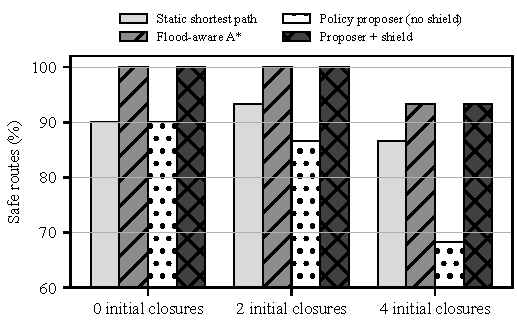
\includegraphics[width=\columnwidth]{fig_safety.pdf}
\caption{Safe-route rate as initial road closures increase (30 seeded scenarios per bar).}
\label{fig:stress}
\end{figure}

Fig.~\ref{fig:stress} shows that the shield matters most when the network is degraded. With four extra closures, the proposer alone fell to 68.3\% safe routes because it kept favouring short routes through roads that had just closed. With the shield, it reached 93.3\%, the same as flood-aware A*. The remaining 6.7\% are scenarios in which no feasible route existed after the closures, so no method could succeed. The flood-severity setting had no measurable effect: across all four values, safe-route rates and capacity violations were identical, and travel times differed by at most 0.01 minutes. The generated flood depths never crossed the 0.75 closure threshold, so closures, not severity, drove the outcome. This exposes a weakness of our scenario generator that we did not see before running the sweep.

Table~\ref{tab:sweep} gives the full sweep. Static shortest path and the risk-aware greedy search behaved identically at every closure level and fell to 86.67\% at four closures. The proposer alone looked faster under heavy closures, with a travel time of 20.47 minutes against 25.27 for the shielded version, but only because some of its routes ran over closed roads. A shorter time on an unsafe route is not a usable result, so travel time should be compared only between methods with the same safe-route rate. Among those, the shield and flood-aware A* were within 0.01 minutes of each other at every level.

\begin{table}[t]
\caption{Safe-route rate (\%) and travel time (min) against initial closures (flood severity 0.35, 30 scenarios each)}
\label{tab:sweep}
\centering
\footnotesize
\setlength{\tabcolsep}{2.6pt}
\begin{tabular}{lcccccc}
\toprule
 & \multicolumn{2}{c}{0 closures} & \multicolumn{2}{c}{2 closures} & \multicolumn{2}{c}{4 closures}\\
Method & Safe & Time & Safe & Time & Safe & Time\\
\midrule
Static shortest path & 90.00 & 16.63 & 93.33 & 18.50 & 86.67 & 24.46\\
Flood-aware A* & 100.00 & 17.81 & 100.00 & 19.31 & 93.33 & 25.28\\
Risk-aware greedy & 90.00 & 16.63 & 93.33 & 18.50 & 86.67 & 24.46\\
Proposer only & 90.00 & 16.63 & 86.67 & 19.07 & 68.33 & 20.47\\
Proposer + shield (SA) & 100.00 & 17.81 & 100.00 & 19.31 & 93.33 & 25.27\\
Proposer + shield (QI) & 100.00 & 17.82 & 100.00 & 19.32 & 93.33 & 25.28\\
\bottomrule
\end{tabular}
\end{table}

A separate ablation on 20 scenarios with a different seed stride ($42+19i$) gave the same picture: 92.5\% safe routes without the shield and 100\% with it, and mean travel time rose from 16.6 to 17.6 minutes. Capacity violations fell from 0.15 per scenario to zero. The shielded pipeline needed slightly more time to re-plan, 2.8 against 2.2 ms in that run, because it scores and filters every candidate before choosing one.

\textit{Worked example.} The first benchmark scenario in which the shield rejected a candidate was seed 93. After the disruption, Shelter A had 10 seats left and group G1 (16 people, vulnerable) needed a route from zone Z1. Table~\ref{tab:shield} lists the proposer's three candidates. The highest-ranked one was the fastest, 16.7 minutes to Shelter A, but would have overfilled it, so the shield rejected it with a capacity violation. The selected route, 23.1 minutes to Shelter B, cost 6.4 minutes more. The explanation shown to the officer lists exactly this: the rejected route, the constraint it broke and the remaining seats.

\begin{table}[t]
\caption{Shield trace for one scenario (seed 93)}
\label{tab:shield}
\centering
\footnotesize
\setlength{\tabcolsep}{3pt}
\begin{tabular}{clccl}
\toprule
Rank & Route & Time (min) & Hazard & Shield\\
\midrule
1 & Z1 $\rightarrow$ A $\rightarrow$ B $\rightarrow$ SA & 16.7 & 0.147 & rejected: capacity\\
2 & Z1 $\rightarrow$ A $\rightarrow$ B $\rightarrow$ E $\rightarrow$ F $\rightarrow$ SB & 23.1 & 0.147 & selected\\
3 & Z1 $\rightarrow$ A $\rightarrow$ D $\rightarrow$ E $\rightarrow$ F $\rightarrow$ SB & 23.5 & 0.206 & feasible\\
\bottomrule
\end{tabular}
\end{table}

\subsection{Reliability Gating}
\label{sec:gating}
We injected each failure type into the base scenario and recorded whether automatic dispatch stayed enabled (Table~\ref{tab:gate}). Only a communications failure, which degrades two sources at once, or three simultaneous failures pushed the mean reliability below 0.60. A complete weather-API outage left the mean at 0.662 and dispatch enabled. Averaging lets four healthy sources hide one failed source, which is the wrong behaviour for a safety gate. We therefore recomputed the gate on the minimum source reliability with the same threshold. It blocked all nine cases with a degraded source, including every single-source failure, and still allowed the healthy case. The margin in the healthy case is zero, however: the idle citizen-report feed sits at exactly 0.60, so a minimum rule needs either per-source thresholds or citizen reports treated as advisory before it can be deployed. The scripted sensor-conflict scenario (flood sensor reporting a flooded road that the road database still lists as open, conflict score 0.71) did block dispatch, as designed.

\begin{table}[t]
\caption{Failure injection: mean-based (deployed) and minimum-based gates, threshold 0.60}
\label{tab:gate}
\centering
\footnotesize
\setlength{\tabcolsep}{3pt}
\begin{tabular}{lcccc}
\toprule
 & \multicolumn{2}{c}{Mean (deployed)} & \multicolumn{2}{c}{Minimum}\\
Injected failure & rel. & dispatch & rel. & dispatch\\
\midrule
None & 0.810 & allowed & 0.600 & allowed\\
Weather API outage & 0.662 & allowed & 0.200 & \textbf{blocked}\\
Delayed radar & 0.744 & allowed & 0.550 & \textbf{blocked}\\
Flood-sensor drift & 0.724 & allowed & 0.480 & \textbf{blocked}\\
Stale road database & 0.746 & allowed & 0.400 & \textbf{blocked}\\
Conflicting citizen reports & 0.780 & allowed & 0.450 & \textbf{blocked}\\
Shelter failure & 0.810 & allowed & 0.600 & allowed\\
Communications failure & 0.586 & \textbf{blocked} & 0.350 & \textbf{blocked}\\
Delayed radar + sensor drift & 0.658 & allowed & 0.480 & \textbf{blocked}\\
Sensor drift + stale roads & 0.660 & allowed & 0.400 & \textbf{blocked}\\
Weather + drift + stale roads & 0.512 & \textbf{blocked} & 0.200 & \textbf{blocked}\\
\bottomrule
\multicolumn{5}{l}{\scriptsize Shelter failure affects capacity, not a data source, and is handled by the shield.}\\
\end{tabular}
\end{table}

\section{Discussion and Limitations}
Three lessons follow from the results. First, a shield is necessary when routes come from a learned or adaptive proposer, but it is not a source of better routes. It brought the proposer back to the level of a well-weighted classical search and no further. The case for a learned proposer therefore has to rest on situations that A* cannot represent, such as congestion that builds over time or many groups competing for the same roads, and our current benchmark does not model either. Second, forecast skill on unseen gauges is high when measured by recall and ranking, but its low precision means that automatic evacuation on the forecast alone would produce many false alarms. Routing the forecast into human review rather than direct action is therefore the right default. Third, how a reliability gate aggregates its inputs matters as much as its threshold.

The per-gauge and threshold results add a practical point. Forecast quality was consistent across catchments, so the main operating decision is the threshold, and Table~\ref{tab:thr} gives an officer the alarm rate to expect at each setting. The feature importances also explain why persistence is a strong baseline and why a forecaster evaluated with random row splits, where neighbouring days of the same flow appear in training, would look even better than ours.

The study has clear limits. The routing network is small and synthetic. Source reliabilities are fixed per status rather than calibrated from data, and the conflict score is scripted. The forecaster is evaluated as a separate service: the live risk score in (\ref{eq:risk}) still uses an earlier model trained on INDOFLOODS as its prior, and replacing it with the gauge forecaster is ongoing work. No field trial or user study with emergency officers has been carried out. Finally, the QAOA-inspired sampler is a classical heuristic and should not be read as evidence about quantum hardware.

We also note threats to the validity of the comparison. All routing methods were run on the same seeded scenarios, so differences between them are not caused by scenario sampling, but they share any bias of the scenario generator, including the flood depths that never crossed the closure threshold. The simulated-annealing and QAOA-inspired solvers pick from the same small feasible set, so their near-identical results say little about either solver. The forecasting gauges are in peninsular India, while the live system serves the Yamuna corridor in the north, so the reported skill may not transfer to that basin. Finally, the safe-route rate is binary per route: it records whether a hard constraint was broken but not how long a group would spend on a hazardous road.

Future work will move the routing benchmark to the Delhi road graph used by the live system. We will also replace the proposer with a trained PPO agent behind the same shield, deploy a minimum-based gate with per-source thresholds, and estimate conflict scores from paired observations.

\section{Conclusion}
We built and evaluated a flood decision-support pipeline that is designed to fail towards human review. On gauges unseen in space and time, a three-day exceedance forecaster detected 90.2\% of flood windows, against 53.8\% for persistence, but with low precision. A QUBO-encoded constraint shield removed every capacity violation from an adaptive route proposer and raised its safe-route rate under heavy closures from 68.3\% to 93.3\%, matching but not beating flood-aware A*. A mean-based reliability gate missed most single-source failures, and a minimum-based gate with the same threshold caught all of them. We report these weaker results because they show which parts of such a system need further work.

\section*{Acknowledgment}
The authors thank the CAMELS-IND and INDOFLOODS dataset authors, Open-Meteo, and the OpenStreetMap contributors for openly available data.
In line with the IEEE policy on AI-generated content, the authors disclose that Claude (Anthropic) was used to help edit and restructure the text of all sections and to draft the plotting and experiment scripts. The experiments use the authors' own software and can be reproduced with fixed seeds. The authors checked every number, claim and reference and take full responsibility for the content.

\balance
\begin{thebibliography}{00}
\bibitem{Nearing2024} G. Nearing \textit{et al.}, ``Global prediction of extreme floods in ungauged watersheds,'' \textit{Nature}, vol. 627, pp. 559--563, 2024.
\bibitem{LiuC2025} C. Liu \textit{et al.}, ``Effective storm surge risk assessment and deep reinforcement learning based evacuation planning: A case study of Daya Bay Petrochemical Industrial Zone,'' \textit{Nat. Hazards Earth Syst. Sci.}, vol. 25, pp. 4767--4786, 2025.
\bibitem{Raei2026} B. Raei, R. Safarzadeh, and X. Wang, ``Congestion-aware multi-agent reinforcement learning for wildfire evacuation routing,'' \textit{Int. Arch. Photogramm. Remote Sens. Spatial Inf. Sci.}, vol. XLIX-M-1-2026, pp. 41--50, 2026.
\bibitem{Alshiekh2018} M. Alshiekh, R. Bloem, R. Ehlers, B. K\"{o}nighofer, S. Niekum, and U. Topcu, ``Safe reinforcement learning via shielding,'' in \textit{Proc. AAAI Conf. Artif. Intell.}, vol. 32, no. 1, 2018, pp. 2669--2678.
\bibitem{Garcia2015} J. Garc\'{i}a and F. Fern\'{a}ndez, ``A comprehensive survey on safe reinforcement learning,'' \textit{J. Mach. Learn. Res.}, vol. 16, pp. 1437--1480, 2015.
\bibitem{Mosavi2018} A. Mosavi, P. Ozturk, and K.-W. Chau, ``Flood prediction using machine learning models: Literature review,'' \textit{Water}, vol. 10, no. 11, Art. no. 1536, 2018.
\bibitem{Kirschstein2024} N. Kirschstein and Y. Sun, ``The merit of river network topology for neural flood forecasting,'' in \textit{Proc. 41st Int. Conf. Mach. Learn. (ICML)}, Vienna, Austria, 2024.
\bibitem{Mangukiya2025} N. K. Mangukiya \textit{et al.}, ``CAMELS-IND: Hydrometeorological time series and catchment attributes for 228 catchments in Peninsular India,'' \textit{Earth Syst. Sci. Data}, vol. 17, pp. 461--491, 2025.
\bibitem{Kuntla2025} S. K. Kuntla and M. Saharia, ``INDOFLOODS: A comprehensive database for flood events in India enhanced with catchment attributes,'' \textit{Bull. Amer. Meteorol. Soc.}, 2025.
\bibitem{Dijkstra1959} E. W. Dijkstra, ``A note on two problems in connexion with graphs,'' \textit{Numer. Math.}, vol. 1, no. 1, pp. 269--271, 1959.
\bibitem{Hart1968} P. E. Hart, N. J. Nilsson, and B. Raphael, ``A formal basis for the heuristic determination of minimum cost paths,'' \textit{IEEE Trans. Syst. Sci. Cybern.}, vol. 4, no. 2, pp. 100--107, 1968.
\bibitem{Yen1971} J. Y. Yen, ``Finding the $k$ shortest loopless paths in a network,'' \textit{Manage. Sci.}, vol. 17, no. 11, pp. 712--716, 1971.
\bibitem{Schulman2017} J. Schulman, F. Wolski, P. Dhariwal, A. Radford, and O. Klimov, ``Proximal policy optimization algorithms,'' arXiv:1707.06347, 2017.
\bibitem{Lucas2014} A. Lucas, ``Ising formulations of many NP problems,'' \textit{Front. Phys.}, vol. 2, Art. no. 5, 2014.
\bibitem{Kirkpatrick1983} S. Kirkpatrick, C. D. Gelatt, and M. P. Vecchi, ``Optimization by simulated annealing,'' \textit{Science}, vol. 220, no. 4598, pp. 671--680, 1983.
\bibitem{Cadelina2024} A. R. Cadeli\~{n}a \textit{et al.}, ``D-Wave implementation of quantum annealing for optimal resource allocation in disaster response operation of Marikina City,'' \textit{ECTI Trans. Comput. Inf. Technol.}, vol. 18, no. 1, pp. 24--33, 2024.
\bibitem{Farhi2014} E. Farhi, J. Goldstone, and S. Gutmann, ``A quantum approximate optimization algorithm,'' arXiv:1411.4028, 2014.
\bibitem{Lundberg2017} S. M. Lundberg and S.-I. Lee, ``A unified approach to interpreting model predictions,'' in \textit{Adv. Neural Inf. Process. Syst. 30}, 2017, pp. 4765--4774.
\bibitem{Lundberg2020} S. M. Lundberg \textit{et al.}, ``From local explanations to global understanding with explainable AI for trees,'' \textit{Nat. Mach. Intell.}, vol. 2, no. 1, pp. 56--67, 2020.
\bibitem{Underhill2026} H. Underhill, L. McEwen, and T. Coulthard, ```That's the dream, right?': Reflections on the co-design of an environmental digital twin by flood risk management professionals,'' \textit{Front. Environ. Sci.}, vol. 13, Art. no. 1724250, 2026.
\bibitem{Chen2016} T. Chen and C. Guestrin, ``XGBoost: A scalable tree boosting system,'' in \textit{Proc. 22nd ACM SIGKDD Int. Conf. Knowl. Discov. Data Min.}, 2016, pp. 785--794.
\end{thebibliography}

\end{document}
